
\documentclass[10pt,a4paper]{article}
\usepackage[margin=1.9cm]{geometry}
\usepackage[T1]{fontenc}
\usepackage[utf8]{inputenc}
\usepackage{lmodern,amsmath,amssymb,booktabs,tabularx,array}
\usepackage{pgfplots}
\pgfplotsset{compat=1.18}
\usepackage{xcolor}
\usepackage[hidelinks]{hyperref}

% Apply a framed, highlighted label to every external hyperlink.
\let\originalhref\href
\renewcommand{\href}[3][]{%
  \originalhref[#1]{#2}{%
    \begingroup
    \setlength{\fboxsep}{2pt}%
    \fcolorbox{blue!60!black}{yellow!25}{\textcolor{blue!60!black}{#3}}%
    \endgroup
  }%
}
\usepackage{microtype}
\usepackage[section]{placeins}

\setlength{\parindent}{0pt}
\setlength{\parskip}{0.35em}
\newcommand{\cm}{\,\mathrm{cm}}
\newcommand{\pct}{\%}
% Round displayed measurements and percentages without changing plot data.
\newcommand{\displaynum}[1]{\pgfmathprintnumber[fixed,fixed zerofill,precision=2,use comma,1000 sep={\,}]{#1}}
\pgfkeys{/pgf/number format/use comma}

\title{Grade 11 C10: Statistical Model of Student Heights}
\author{Nicolas Olando Lopez\\
	11 -- Example \quad | \quad Global Economics 2026--2027}
\date{2 November 2026}

\begin{document}
	\maketitle
	\vspace{-2em}
	
	\section{Choose a question and obtain data}
\textbf{Question.} What proportion of surveyed students is taller than
	180 cm, and how might the estimate inform preliminary school-uniform
	inventory planning? The 180 cm cutoff is illustrative, not an official
	uniform specification. Height alone does not determine clothing size.
	
	Let $X$ denote a student's recorded height in centimeters. It is
	treated as continuous, although reported measurements may be rounded.
	
	\begin{table}[htbp]
		\centering
		\caption{Dataset summary}
		\label{tab:data}
		\renewcommand{\arraystretch}{1.5}
		\begin{tabularx}{\linewidth}{@{}p{3.6cm}X@{}}
			\toprule
			Characteristic & Value \\
			\midrule
			Data source &
			\href{https://correosanbartoloedu-my.sharepoint.com/:x:/g/personal/nicolas_lopez_sanbartolo_edu_co/IQCNZmoI8AlsTLMhGQnIz8V5AbLzWOtFlaSgxntvIurVxRA?e=XgwWFs}{Manually entered survey dataset} \\
			Variable &
			Recorded height (cm) \\
			Observations &
			$n=109$ numerical values \\
			Observed range &
			151--191 cm; sample extrema, not population bounds \\
			\bottomrule
		\end{tabularx}
	\end{table}
	
	\textbf{Data reference.}
	\href{https://correosanbartoloedu-my.sharepoint.com/:x:/g/personal/nicolas_lopez_sanbartolo_edu_co/IQCNZmoI8AlsTLMhGQnIz8V5AbLzWOtFlaSgxntvIurVxRA?e=XgwWFs}
	{Manually entered survey dataset}.

\section{Summarise the data}
For observations $x_1,\ldots,x_n$, the sample statistics use
	denominator $n-1$:
	\[
	\bar x=\frac{\sum x_i}{n},\qquad
	s^2=\frac{\sum(x_i-\bar x)^2}{n-1},\qquad
	s=\sqrt{s^2}.
	\]
	
	\begin{table}[htbp]
		\centering
		\caption{Observed totals and sample statistics}
		\label{tab:summary}
		\renewcommand{\arraystretch}{1.5}
		\begin{tabular}{@{}lll@{}}
			\toprule
			Quantity & Calculation & Result \\
			\midrule
			$n$ & All retained records & $109$ \\
			$\sum x_i$ & Direct sum & $\displaynum{18482.5}\cm$ \\
			$\sum x_i^2$ & Direct sum &
			$\displaynum{3142981.25}\,\mathrm{cm}^2$ \\
			$\sum(x_i-\bar x)^2$ &
			$\displaynum{3142981.25}-(\displaynum{18482.5})^2/109$ &
			$\displaynum{9010.550459}\,\mathrm{cm}^2$ \\
			$\bar x$ & $\displaynum{18482.5}/109$ & $\displaynum{169.564220}\cm$ \\
			$s^2$ & $\displaynum{9010.550459}/108$ &
			$\displaynum{83.431023}\,\mathrm{cm}^2$ \\
			$s$ & $\sqrt{\displaynum{83.431023}}$ & $\displaynum{9.134058}\cm$ \\
			\bottomrule
		\end{tabular}
	\end{table}
	

	
	
	
	
\begin{figure}[htbp]
\centering
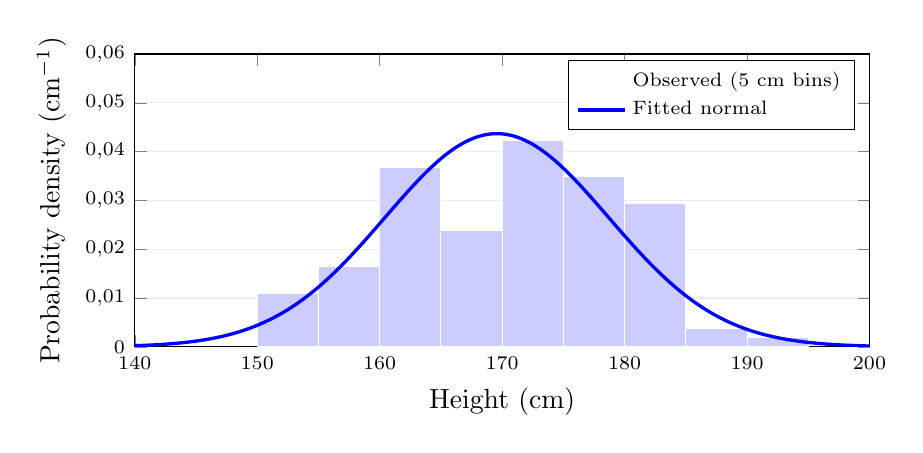
\begin{tikzpicture}
\begin{axis}[width=.9\linewidth,height=5.3cm,
xmin=140,xmax=200,ymin=0,ymax=.060,
xtick={140,150,160,170,180,190,200},ytick={0,.01,.02,.03,.04,.05,.06},
scaled y ticks=false,yticklabel style={/pgf/number format/fixed},
xlabel={Height (cm)},ylabel={Probability density ($\mathrm{cm}^{-1}$)},
tick label style={font=\scriptsize},ymajorgrids,grid style={gray!15},
legend style={at={(.98,.98)},anchor=north east,font=\scriptsize,cells={anchor=west}}]
\addplot[ybar interval,fill=blue!20,draw=white] coordinates {
(150,0.0110091743119) (155,0.0165137614679) (160,0.0366972477064) (165,0.0238532110092) (170,0.0422018348624) (175,0.0348623853211) (180,0.0293577981651) (185,0.00366972477064) (190,0.00183486238532) (195,0)};
\addlegendentry{Observed (5 cm bins)}
\addplot[very thick,blue,domain=140:200,samples=200] {exp(-((x-169.564220183486)^2)/(2*9.13405839514316^2))/(9.13405839514316*sqrt(2*pi))};\addlegendentry{Fitted normal}
\end{axis}
\end{tikzpicture}
\caption{Sample-SD normal fit over the observed histogram.
Bins are $[150,155),\ldots,[190,195)$; each bar height is its count divided by $109\times5$.
Bars have total area one; curves and bars share density units.
Both density overlays use identical axes and bins.}
\label{fig:density}
\end{figure}

\section{Select and fit one probability density function}
The 5 cm histogram in Figure~\ref{fig:density} is irregular and not perfectly symmetric.
	Following the assignment's specified normal-estimation rule,
	$\widehat\mu=\bar x$ and $\widehat\sigma=s>0$.
	
	\[
	X\sim N(\displaynum{169.564220}\cm,\;\displaynum{83.431023}\,\mathrm{cm}^2),
	\]
	\[
	f(x)=\frac{1}{\displaynum{9.134058}\sqrt{2\pi}}
	\exp\!\left[
	-\frac{(x-\displaynum{169.564220})^2}{2(\displaynum{9.134058})^2}
	\right].
	\]
	
	Here $x$ is the numerical height in cm, $f(x)$ has units
	$\mathrm{cm}^{-1}$, and the support is $(-\infty,\infty)$.
	


	
	\begin{table}[htbp]
		\centering
		\caption{Model parameters and moment comparison}
		\label{tab:moments}
		\renewcommand{\arraystretch}{1.5}
		\begin{tabular}{@{}lrrl@{}}
			\toprule
			Quantity & Sample & Fitted normal & Units \\
			\midrule
			Mean & \displaynum{169.564220} & \displaynum{169.564220} & cm \\
			Variance & \displaynum{83.431023} & \displaynum{83.431023} & $\mathrm{cm}^2$ \\
			Standard deviation & \displaynum{9.134058} & \displaynum{9.134058} & cm \\
			\bottomrule
		\end{tabular}
	\end{table}
	
	\begin{figure}[htbp]
		\centering
		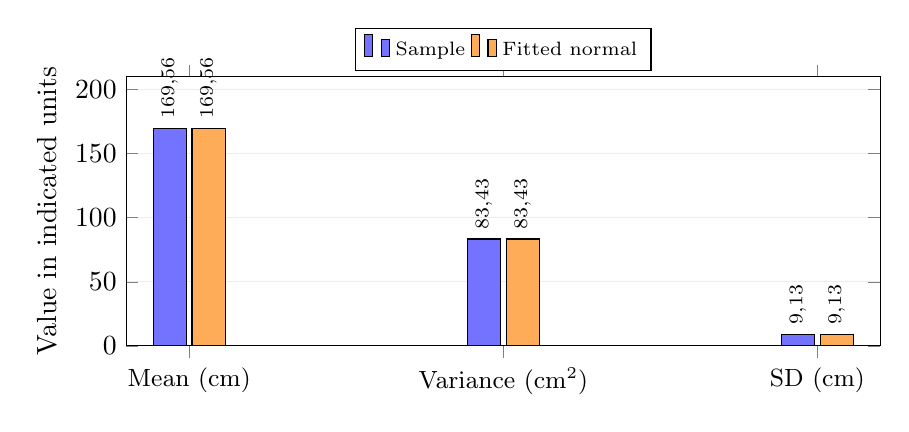
\begin{tikzpicture}
			\begin{axis}[
				width=.92\linewidth,
				height=5cm,
				ybar,
				bar width=12pt,
				ymin=0,ymax=210,
				xtick={1,2,3},
				xticklabels={Mean (cm),Variance ($\mathrm{cm}^2$),SD (cm)},
				xticklabel style={font=\small},
				ylabel={Value in indicated units},
				ytick={0,50,100,150,200},
				legend style={
					at={(.5,1.02)},
					anchor=south,
					legend columns=2,
					font=\scriptsize
				},
				node near coords style={
					font=\scriptsize,
					rotate=90,
					anchor=west,
					/pgf/number format/.cd,fixed,fixed zerofill,precision=2
				},
				nodes near coords,
				ymajorgrids,
				grid style={gray!15}
				]
				\addplot[fill=blue!55] coordinates {
					(1,169.564220)
					(2,83.431023)
					(3,9.134058)
				};
				\addplot[fill=orange!65] coordinates {
					(1,169.564220)
					(2,83.431023)
					(3,9.134058)
				};
				\legend{Sample,Fitted normal}
			\end{axis}
		\end{tikzpicture}
		\caption{Paired sample--model moments: equal by parameter
			estimation, not independent evidence of fit. Bar labels are
			rounded to two decimal places, as in
			Table~\ref{tab:moments}. Each category uses the
			units indicated on the horizontal axis.}
		\label{fig:moments}
	\end{figure}

\section{Calculate quantiles and model probabilities}
Write $\Phi$ for the standard-normal CDF. With
	$z_{0.10}=-1.2815515655$ and $z_{0.90}=1.2815515655$,
	
	\[
	q_p=\widehat\mu+\widehat\sigma z_p,
	\]
	\[
	q_{0.10}
	=\displaynum{169.564220}+\displaynum{9.134058}(-1.2815515655)
	=\displaynum{157.858453}\cm,
	\]
	\[
	q_{0.90}
	=\displaynum{169.564220}+\displaynum{9.134058}(1.2815515655)
	=\displaynum{181.269987}\cm.
	\]
	
	The unrounded fitted quantiles imply model probabilities
	$0.10$, $0.80$, and $0.10$ by construction. Endpoints
	have probability zero.
	
	For empirical comparisons, the fixed cutoffs (rounded for display) are
	$a=\displaynum{157.858453}\cm$, $b=\displaynum{181.269987}\cm$ and
	$c=\displaynum{180.000000}\cm$. All model probabilities below are
	evaluated at \emph{these same numerical cutoffs}, using
	the full-precision fitted moments.
	
	\[
	P(X<c)=\Phi\!\left(
	\frac{c-\widehat\mu}{\widehat\sigma}
	\right),
	\]
	\[
	P(X>180)
	=1-\Phi\!\left(
	\frac{180-\displaynum{169.564220}}{\displaynum{9.134058}}
	\right)
	=0.126620437.
	\]

\section{Compare empirical and model probabilities}
\begin{table}[htbp]
		\centering
		\caption{Observed versus fitted probabilities at identical
			boundaries (cm)}
		\label{tab:prob}
		\setlength{\tabcolsep}{3pt}
		\begin{tabularx}{\linewidth}{
				@{}>{\raggedright\arraybackslash}Xrrrrrr@{}}
			\toprule
			Event (cm) & Count & $n$ & Empirical & Model &
			Absolute & Error (\%) \\
			\midrule
			$X<\displaynum{157.858453}$ &
			10 & 109 & 0.091743 & 0.100000 & 0.008257 & \displaynum{8.26} \\
			$\displaynum{157.858453}\le X\le\displaynum{181.269987}$ &
			91 & 109 & 0.834862 & 0.800000 & 0.034862 & \displaynum{4.36} \\
			$X>\displaynum{181.269987}$ &
			8 & 109 & 0.073394 & 0.100000 & 0.026606 & \displaynum{26.61} \\
			$X>\displaynum{180.000000}$ &
			13 & 109 & 0.119266 & 0.126620 & 0.007354 & \displaynum{5.81} \\
			\bottomrule
		\end{tabularx}
	\end{table}
	
	\begin{figure}[htbp]
		\centering
		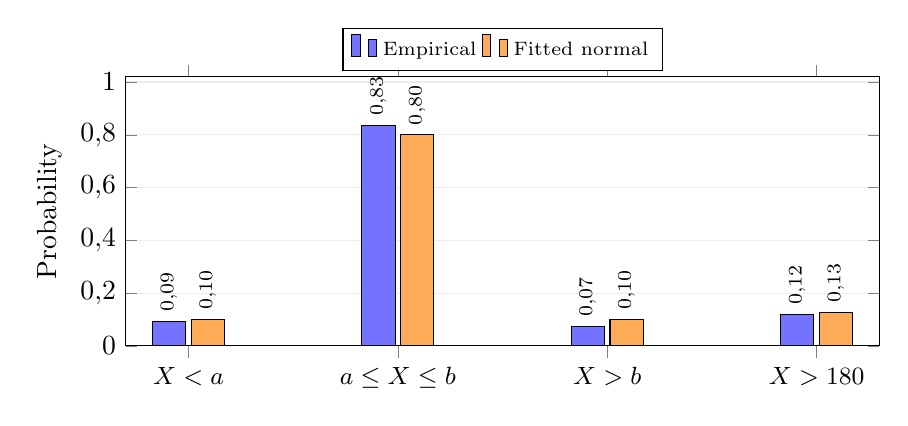
\begin{tikzpicture}
			\begin{axis}[
				width=.92\linewidth,
				height=5cm,
				ybar,
				bar width=12pt,
				ymin=0,ymax=1.02,
				xtick={1,2,3,4},
				xticklabels={
					$X<a$,
					$a\le X\le b$,
					$X>b$,
					$X>180$
				},
				xticklabel style={font=\small},
				ylabel={Probability},
				ytick={0,.2,.4,.6,.8,1},
				legend style={
					at={(.5,1.02)},
					anchor=south,
					legend columns=2,
					font=\scriptsize
				},
				node near coords style={
					font=\scriptsize,
					rotate=90,
					anchor=west,
					/pgf/number format/.cd,fixed,fixed zerofill,precision=2
				},
				nodes near coords,
				ymajorgrids,
				grid style={gray!15}
				]
				\addplot[fill=blue!55] coordinates {
					(1,0.091743119)
					(2,0.834862385)
					(3,0.073394495)
					(4,0.119266055)
				};
				\addplot[fill=orange!65] coordinates {
					(1,0.099999993)
					(2,0.800000006)
					(3,0.100000000)
					(4,0.126620437)
				};
				\legend{Empirical,Fitted normal}
			\end{axis}
		\end{tikzpicture}
		\caption{Paired empirical and model probabilities,
			with matching event definitions. Values are rounded to
			two decimals in the bar labels; Table~\ref{tab:prob}
			retains six decimals.}
		\label{fig:probs}
	\end{figure}
	
	Counts are based on individual observations, not histogram
	bins or sample percentiles. The first three disjoint event
	counts satisfy $10+91+8=109$; the fourth event overlaps them.
	
	For an event $A$ with count $k_A$,
	
	\[
	p_{\mathrm{emp}}=\frac{k_A}{109},\quad
	\mathrm{EA}=|p_{\mathrm{emp}}-p_{\mathrm{model}}|,
	\quad
	E_{\%}=100\frac{\mathrm{EA}}{|p_{\mathrm{model}}|}\%.
	\]
	
	For the first event,
	$\mathrm{EA}=|10/109-0.099999993325|=0.008256874$
	and $E_{\%}=\displaynum{8.26}\%$.
	
	The difference is $\displaynum{0.826}$ percentage points,
	distinct from the relative percentage error.
	No model probability is zero.
	

	\begin{figure}[htbp]
		\centering
		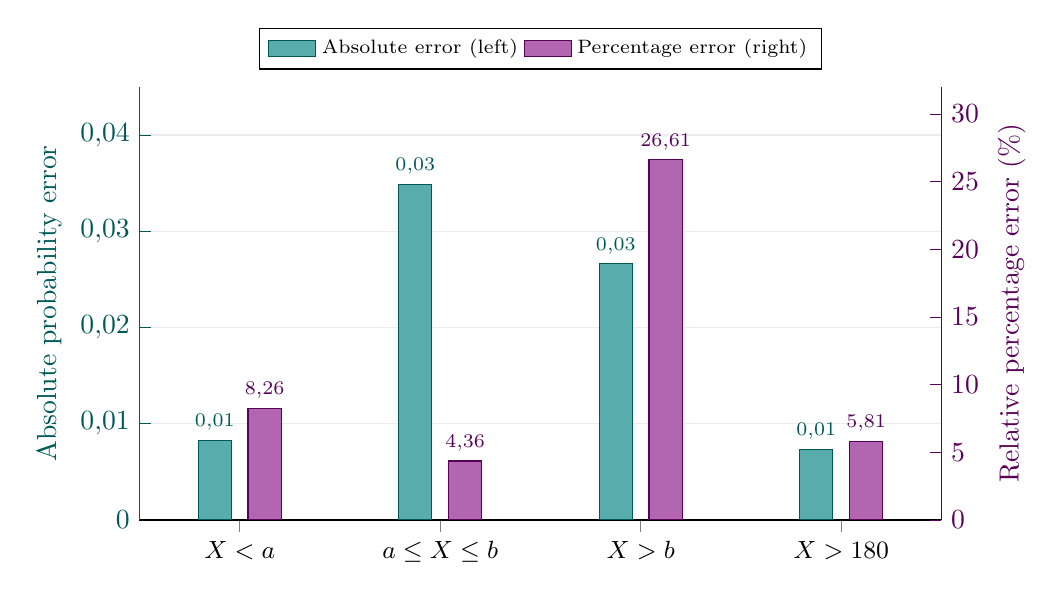
\begin{tikzpicture}
			\begin{axis}[
				width=.84\linewidth,height=5.5cm,
				scale only axis,
				xmin=.5,xmax=4.5,
				ymin=0,ymax=.045,
				axis y line*=left,
				axis x line*=bottom,
				xtick={1,2,3,4},
				xticklabels={$X<a$,$a\le X\le b$,$X>b$,$X>180$},
				xticklabel style={font=\small},
				ylabel={Absolute probability error},
				ytick={0,.01,.02,.03,.04},
				scaled y ticks=false,
				y axis line style={teal!70!black},
				y tick style={teal!70!black},
				yticklabel style={text=teal!70!black,/pgf/number format/fixed},
				ylabel style={text=teal!70!black},
				ybar,bar width=12pt,bar shift=-9pt,
				nodes near coords,
				node near coords style={
					font=\scriptsize,text=teal!70!black,
					/pgf/number format/.cd,fixed,fixed zerofill,precision=2
				},
				ymajorgrids,grid style={gray!15},
				legend style={at={(.5,1.04)},anchor=south,
					legend columns=2,font=\scriptsize}
				]
				\addplot[area legend,fill=teal!65,draw=teal!70!black] coordinates {
					(1,.008256874059)
					(2,.034862379321)
					(3,.026605504587)
					(4,.007354381954)
				};
				\addlegendentry{Absolute error (left)}
				\addlegendimage{area legend,fill=violet!60,draw=violet!70!black}
				\addlegendentry{Percentage error (right)}
			\end{axis}
			\begin{axis}[
				width=.84\linewidth,height=5.5cm,
				scale only axis,
				xmin=.5,xmax=4.5,
				ymin=0,ymax=32,
				axis y line*=right,
				axis x line=none,
				xtick=\empty,
				ylabel={Relative percentage error (\%)},
				ytick={0,5,10,15,20,25,30},
				scaled y ticks=false,
				y axis line style={violet!70!black},
				y tick style={violet!70!black},
				yticklabel style={text=violet!70!black,/pgf/number format/fixed},
				ylabel style={text=violet!70!black},
				ybar,bar width=12pt,bar shift=9pt,
				nodes near coords,
				node near coords style={
					font=\scriptsize,text=violet!70!black,
					/pgf/number format/.cd,fixed,fixed zerofill,precision=2
				}
				]
				\addplot[fill=violet!60,draw=violet!70!black] coordinates {
					(1,8.256874610091)
					(2,4.357797382454)
					(3,26.605504587156)
					(4,5.808210845243)
				};
			\end{axis}
		\end{tikzpicture}
		\caption{Errors for the four events in Table~\ref{tab:prob}.
			Teal bars and the left scale show absolute probability errors;
			violet bars and the right scale show relative percentage errors.
			Bar heights use unrounded values; labels show two decimal places.}
		\label{fig:errors}
	\end{figure}

	This comparison implements C6 (relative frequencies
	versus theoretical probabilities); the equality of sample
	and fitted moments implements the estimation convention
	used in C7, not an independent model check.

\section{Interpret the results}
The fitted normal probability of height above 180 cm is
	$0.126620$ (\displaynum{12.66}\%); the observed frequency is
	$13/109=0.119266$ (\displaynum{11.93}\%). The descriptive mixture gives
	$0.114421$ (\displaynum{11.44}\%). Both are plausible in-sample approximations;
	the mixture is closer at this cutoff, which alone does not establish
	better prediction for new students.
	
	For the normal model, the unique largest absolute difference occurs at
	$\displaynum{157.858453}\le X\le\displaynum{181.269987}\cm$:
	$0.034862$ (\displaynum{3.49} percentage points).
	Imperfect symmetry or student-subgroup heterogeneity
	may contribute, but neither is established as the cause.
	
	\begin{table}[htbp]
		\centering
		\caption{Principal limitations}
		\label{tab:limits}
		\renewcommand{\arraystretch}{1.5}
		\begin{tabularx}{\linewidth}{@{}p{3.1cm}X@{}}
			\toprule
			Issue & Implication \\
			\midrule
			Sampling / measurement &
			Unknown selection and recording procedures limit
			population generalization. \\
			Model support / shape &
			The normal density permits impossible negative or
			arbitrarily large heights; histogram symmetry is imperfect. \\
			Operational applicability &
			The 180 cm cutoff is hypothetical; height alone does not
			determine uniform size. \\
			In-sample evaluation &
			The same 109 records fit and assess the model; agreement
			does not establish predictive accuracy for new students. \\
			\bottomrule
		\end{tabularx}
	\end{table}

\section{Register AI use}
\href{https://chatgpt.com/s/cx_6ae90c6e64c48191895b214d2ec1325e}{Conversation 1}
	
	\href{https://chatgpt.com/share/6ae90c7e-883c-83e9-a109-417007a893d4}{Conversation 2}
	
	\href{https://chatgpt.com/share/6ae90d1d-535c-83e9-a1e7-e38b6d64715b}{Conversation 3}
	
	\href{https://chatgpt.com/share/6ae90ddf-76f4-83e9-a03f-39b384abf9c9}{Conversation 4}
	
	\href{https://chatgpt.com/s/cx_6ae91036e6ac819198538e259cb8ca30}{Conversation 5}

\section{Brief extension: two-component skew-normal mixture}
As a descriptive alternative, use the already fitted model in
\texttt{assets/data/heights.tex}, with full-precision parameters and quantiles
from \texttt{heights\_results.json}; no model is refitted here.
It combines two curves, with weights adding to one:
\[
 f_M(x)=\sum_{j=1}^{2}w_j\frac{2}{\omega_j}\phi(z_j)\Phi(\alpha_jz_j),
 \qquad z_j=\frac{x-\xi_j}{\omega_j}.
\]
Here $\phi$ and $\Phi$ are the standard-normal density and CDF;
$\xi$ is location, $\omega>0$ is scale, and $\alpha$ controls skewness.
Skew-normal location and scale are generally \emph{not} the component
mean and SD. For example, component 1 has mean \displaynum{160.9511} cm and SD
\displaynum{4.7685} cm, despite its different location and scale below.

\begin{table}[htbp]
\centering
\caption{Mixture parameters (rounded only for display)}\label{tab:mixparams}
\renewcommand{\arraystretch}{1.5}
\begin{tabular}{@{}lrrrr@{}}\toprule
Component & Weight $w$ & Location $\xi$ (cm) & Scale $\omega$ (cm) & Shape $\alpha$\\\midrule
1 & 0.444318 & \displaynum{166.734909} & \displaynum{7.496063} & -3.797348\\
2 & 0.555682 & \displaynum{169.598283} & \displaynum{8.223408} & 20.000000\\
\bottomrule\end{tabular}
\end{table}

\begin{table}[htbp]
\centering
\caption{Sample and fitted-model moments}\label{tab:mixmoments}
\renewcommand{\arraystretch}{1.5}
\begin{tabular}{@{}lrrr@{}}\toprule
Quantity & Sample & Fitted normal & Fitted mixture\\\midrule
Mean (cm) & \displaynum{169.564220} & \displaynum{169.564220} & \displaynum{169.397656}\\
Variance ($\mathrm{cm}^2$) & \displaynum{83.431023} & \displaynum{83.431023} & \displaynum{80.863867}\\
SD (cm) & \displaynum{9.134058} & \displaynum{9.134058} & \displaynum{8.992434}\\
\bottomrule\end{tabular}
\end{table}
The sample variance uses $n-1$; model variances are distribution moments.
The normal column uses the main task's sample-SD rule. The source's
model-selection table instead uses the maximum-likelihood normal SD
($\sqrt{\sum(x_i-\bar x)^2/n}$). Among its candidate models, AIC favors
two normals and BIC favors a single normal; neither selects this mixture.

\begin{figure}[htbp]
\centering
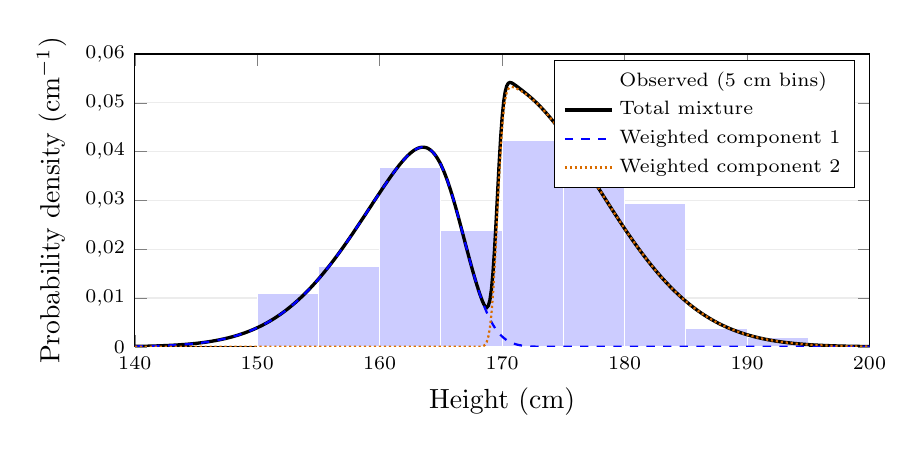
\begin{tikzpicture}
\begin{axis}[width=.9\linewidth,height=5.3cm,
xmin=140,xmax=200,ymin=0,ymax=.060,
xtick={140,150,160,170,180,190,200},ytick={0,.01,.02,.03,.04,.05,.06},
scaled y ticks=false,yticklabel style={/pgf/number format/fixed},
xlabel={Height (cm)},ylabel={Probability density ($\mathrm{cm}^{-1}$)},
tick label style={font=\scriptsize},ymajorgrids,grid style={gray!15},
legend style={at={(.98,.98)},anchor=north east,font=\scriptsize,cells={anchor=west}}]
\addplot[ybar interval,fill=blue!20,draw=white] coordinates {
(150,0.0110091743119) (155,0.0165137614679) (160,0.0366972477064) (165,0.0238532110092) (170,0.0422018348624) (175,0.0348623853211) (180,0.0293577981651) (185,0.00366972477064) (190,0.00183486238532) (195,0)};
\addlegendentry{Observed (5 cm bins)}
\addplot[very thick,black] coordinates {
(140.000,8.178297252e-05) (140.125,8.678235859e-05) (140.250,9.206175356e-05) (140.375,9.763516678e-05) (140.500,0.0001035172051) (140.625,0.0001097230924) (140.750,0.0001162686892) (140.875,0.0001231705128) (141.000,0.0001304457573) (141.125,0.0001381123145) (141.250,0.0001461887943) (141.375,0.0001546945455) (141.500,0.0001636496773) (141.625,0.0001730750803) (141.750,0.0001829924476) (141.875,0.0001934242967) (142.000,0.0002043939904) (142.125,0.0002159257588) (142.250,0.0002280447206) (142.375,0.0002407769042) (142.500,0.0002541492696) (142.625,0.000268189729) (142.750,0.0002829271683) (142.875,0.0002983914675) (143.000,0.0003146135213) (143.125,0.0003316252594) (143.250,0.0003494596663) (143.375,0.0003681508002) (143.500,0.0003877338126) (143.625,0.0004082449661) (143.750,0.0004297216523) (143.875,0.0004522024088) (144.000,0.0004757269356) (144.125,0.0005003361105) (144.250,0.0005260720037) (144.375,0.0005529778917) (144.500,0.0005810982698) (144.625,0.0006104788638) (144.750,0.0006411666402) (144.875,0.0006732098158) (145.000,0.0007066578653) (145.125,0.0007415615279) (145.250,0.0007779728121) (145.375,0.0008159449994) (145.500,0.0008555326459) (145.625,0.0008967915825) (145.750,0.0009397789133) (145.875,0.0009845530115) (146.000,0.001031173514) (146.125,0.001079701315) (146.250,0.001130198552) (146.375,0.001182728601) (146.500,0.001237356053) (146.625,0.001294146706) (146.750,0.00135316754) (146.875,0.001414486697) (147.000,0.001478173456) (147.125,0.001544298206) (147.250,0.001612932417) (147.375,0.001684148605) (147.500,0.001758020299) (147.625,0.001834621998) (147.750,0.001914029133) (147.875,0.001996318019) (148.000,0.002081565809) (148.125,0.00216985044) (148.250,0.00226125058) (148.375,0.002355845569) (148.500,0.002453715354) (148.625,0.002554940431) (148.750,0.00265960177) (148.875,0.002767780743) (149.000,0.002879559054) (149.125,0.002995018653) (149.250,0.003114241655) (149.375,0.003237310256) (149.500,0.003364306641) (149.625,0.003495312888) (149.750,0.003630410878) (149.875,0.003769682185) (150.000,0.003913207979) (150.125,0.004061068916) (150.250,0.004213345026) (150.375,0.004370115602) (150.500,0.004531459076) (150.625,0.004697452907) (150.750,0.00486817345) (150.875,0.005043695833) (151.000,0.005224093826) (151.125,0.005409439707) (151.250,0.005599804133) (151.375,0.005795255993) (151.500,0.005995862277) (151.625,0.006201687928) (151.750,0.0064127957) (151.875,0.00662924601) (152.000,0.006851096794) (152.125,0.007078403355) (152.250,0.007311218211) (152.375,0.007549590947) (152.500,0.007793568059) (152.625,0.008043192803) (152.750,0.008298505041) (152.875,0.008559541086) (153.000,0.00882633355) (153.125,0.00909891119) (153.250,0.009377298754) (153.375,0.009661516832) (153.500,0.009951581706) (153.625,0.0102475052) (153.750,0.01054929452) (153.875,0.01085695213) (154.000,0.01117047561) (154.125,0.0114898575) (154.250,0.01181508515) (154.375,0.01214614064) (154.500,0.01248300058) (154.625,0.01282563605) (154.750,0.01317401243) (154.875,0.01352808931) (155.000,0.01388782037) (155.125,0.01425315326) (155.250,0.01462402953) (155.375,0.0150003845) (155.500,0.0153821472) (155.625,0.01576924026) (155.750,0.01616157987) (155.875,0.01655907566) (156.000,0.01696163069) (156.125,0.01736914137) (156.250,0.01778149741) (156.375,0.01819858179) (156.500,0.01862027072) (156.625,0.01904643362) (156.750,0.01947693311) (156.875,0.01991162499) (157.000,0.02035035821) (157.125,0.02079297492) (157.250,0.02123931046) (157.375,0.02168919332) (157.500,0.0221424452) (157.625,0.02259888102) (157.750,0.02305830885) (157.875,0.02352052998) (158.000,0.02398533883) (158.125,0.02445252297) (158.250,0.02492186296) (158.375,0.0253931323) (158.500,0.02586609725) (158.625,0.0263405166) (158.750,0.02681614135) (158.875,0.02729271434) (159.000,0.02776996974) (159.125,0.02824763234) (159.250,0.02872541683) (159.375,0.02920302668) (159.500,0.029680153) (159.625,0.030156473) (159.750,0.03063164819) (159.875,0.03110532231) (160.000,0.03157711881) (160.125,0.03204663795) (160.250,0.03251345347) (160.375,0.03297710882) (160.500,0.03343711278) (160.625,0.03389293472) (160.750,0.0343439992) (160.875,0.03478968013) (161.000,0.03522929448) (161.125,0.03566209539) (161.250,0.03608726513) (161.375,0.03650390755) (161.500,0.03691104057) (161.625,0.03730758849) (161.750,0.03769237462) (161.875,0.03806411424) (162.000,0.03842140818) (162.125,0.03876273743) (162.250,0.03908645889) (162.375,0.03939080273) (162.500,0.03967387166) (162.625,0.03993364246) (162.750,0.04016797011) (162.875,0.04037459483) (163.000,0.04055115245) (163.125,0.04069518815) (163.250,0.04080417401) (163.375,0.04087553028) (163.500,0.0409066506) (163.625,0.04089493097) (163.750,0.04083780238) (163.875,0.04073276673) (164.000,0.04057743576) (164.125,0.04036957226) (164.250,0.04010713312) (164.375,0.03978831319) (164.500,0.0394115893) (164.625,0.03897576332) (164.750,0.03848000331) (164.875,0.03792388163) (165.000,0.03730740898) (165.125,0.0366310634) (165.250,0.03589581301) (165.375,0.0351031319) (165.500,0.03425500819) (165.625,0.03335394375) (165.750,0.03240294514) (165.875,0.03140550558) (166.000,0.03036557796) (166.125,0.02928753911) (166.250,0.0281761459) (166.375,0.02703648375) (166.500,0.02587390862) (166.625,0.02469398341) (166.750,0.02350241033) (166.875,0.02230496023) (167.000,0.02110740075) (167.125,0.01991542463) (167.250,0.01873457976) (167.375,0.01757020291) (167.500,0.01642736025) (167.625,0.01531080281) (167.750,0.01422496268) (167.875,0.0131740674) (168.000,0.01216258155) (168.125,0.01119646423) (168.250,0.01028620185) (168.375,0.009453113241) (168.500,0.008740506342) (168.625,0.008229874487) (168.750,0.008058410826) (168.875,0.008428006902) (169.000,0.009590895482) (169.125,0.01179932868) (169.250,0.0152210401) (169.375,0.01984573183) (169.500,0.02542660381) (169.625,0.03149749674) (169.750,0.03747458569) (169.875,0.04280725994) (170.000,0.0471148092) (170.125,0.05025375101) (170.250,0.05229913926) (170.375,0.05346526469) (170.500,0.05401134229) (170.625,0.05416995835) (170.750,0.05411302708) (170.875,0.05394932365) (171.000,0.05373872808) (171.125,0.05350998983) (171.250,0.05327493213) (171.375,0.0530373875) (171.500,0.05279790652) (171.625,0.05255589587) (171.750,0.05231046647) (171.875,0.05206072827) (172.000,0.05180587806) (172.125,0.05154521871) (172.250,0.05127815816) (172.375,0.0510042029) (172.500,0.05072295013) (172.625,0.05043407971) (172.750,0.05013734627) (172.875,0.04983257158) (173.000,0.04951963739) (173.125,0.04919847861) (173.250,0.04886907708) (173.375,0.04853145583) (173.500,0.04818567388) (173.625,0.04783182149) (173.750,0.047470016) (173.875,0.04710039808) (174.000,0.04672312842) (174.125,0.04633838484) (174.250,0.0459463598) (174.375,0.04554725813) (174.500,0.04514129521) (174.625,0.04472869527) (174.750,0.04430968998) (174.875,0.04388451725) (175.000,0.04345342015) (175.125,0.04301664604) (175.250,0.04257444571) (175.375,0.04212707277) (175.500,0.04167478298) (175.625,0.0412178338) (175.750,0.04075648382) (175.875,0.04029099242) (176.000,0.03982161934) (176.125,0.03934862437) (176.250,0.03887226698) (176.375,0.03839280605) (176.500,0.03791049962) (176.625,0.03742560454) (176.750,0.03693837631) (176.875,0.0364490688) (177.000,0.035957934) (177.125,0.03546522186) (177.250,0.03497118003) (177.375,0.03447605366) (177.500,0.03398008524) (177.625,0.03348351436) (177.750,0.0329865776) (177.875,0.03248950827) (178.000,0.0319925363) (178.125,0.03149588808) (178.250,0.03099978628) (178.375,0.0305044497) (178.500,0.03001009317) (178.625,0.02951692737) (178.750,0.02902515873) (178.875,0.0285349893) (179.000,0.02804661665) (179.125,0.02756023376) (179.250,0.02707602891) (179.375,0.02659418559) (179.500,0.02611488244) (179.625,0.02563829315) (179.750,0.02516458639) (179.875,0.02469392576) (180.000,0.02422646972) (180.125,0.02376237157) (180.250,0.02330177936) (180.375,0.0228448359) (180.500,0.02239167869) (180.625,0.02194243993) (180.750,0.02149724651) (180.875,0.02105621997) (181.000,0.02061947651) (181.125,0.020187127) (181.250,0.01975927698) (181.375,0.01933602669) (181.500,0.01891747107) (181.625,0.01850369981) (181.750,0.01809479734) (181.875,0.01769084293) (182.000,0.01729191068) (182.125,0.0168980696) (182.250,0.01650938363) (182.375,0.01612591172) (182.500,0.01574770789) (182.625,0.0153748213) (182.750,0.01500729629) (182.875,0.01464517248) (183.000,0.01428848486) (183.125,0.01393726381) (183.250,0.01359153526) (183.375,0.01325132073) (183.500,0.01291663743) (183.625,0.01258749834) (183.750,0.01226391233) (183.875,0.01194588424) (184.000,0.011633415) (184.125,0.01132650167) (184.250,0.01102513764) (184.375,0.01072931264) (184.500,0.0104390129) (184.625,0.01015422126) (184.750,0.009874917232) (184.875,0.00960107716) (185.000,0.009332674296) (185.125,0.009069678926) (185.250,0.008812058472) (185.375,0.008559777608) (185.500,0.008312798365) (185.625,0.008071080246) (185.750,0.007834580332) (185.875,0.007603253395) (186.000,0.007377052003) (186.125,0.007155926632) (186.250,0.006939825771) (186.375,0.006728696029) (186.500,0.006522482239) (186.625,0.006321127566) (186.750,0.006124573606) (186.875,0.005932760489) (187.000,0.00574562698) (187.125,0.005563110574) (187.250,0.005385147599) (187.375,0.005211673305) (187.500,0.005042621959) (187.625,0.004877926939) (187.750,0.004717520821) (187.875,0.004561335467) (188.000,0.004409302108) (188.125,0.004261351434) (188.250,0.004117413667) (188.375,0.003977418647) (188.500,0.003841295902) (188.625,0.00370897473) (188.750,0.003580384263) (188.875,0.003455453545) (189.000,0.003334111593) (189.125,0.003216287467) (189.250,0.00310191033) (189.375,0.00299090951) (189.500,0.002883214557) (189.625,0.002778755301) (189.750,0.002677461905) (189.875,0.002579264913) (190.000,0.002484095305) (190.125,0.00239188454) (190.250,0.002302564599) (190.375,0.00221606803) (190.500,0.00213232799) (190.625,0.002051278277) (190.750,0.001972853369) (190.875,0.001896988458) (191.000,0.001823619482) (191.125,0.001752683151) (191.250,0.001684116978) (191.375,0.001617859302) (191.500,0.001553849314) (191.625,0.001492027075) (191.750,0.001432333541) (191.875,0.001374710575) (192.000,0.001319100968) (192.125,0.00126544845) (192.250,0.001213697707) (192.375,0.001163794388) (192.500,0.001115685116) (192.625,0.0010693175) (192.750,0.001024640134) (192.875,0.0009816026119) (193.000,0.0009401555229) (193.125,0.0009002504597) (193.250,0.0008618400179) (193.375,0.0008248777965) (193.500,0.0007893183974) (193.625,0.0007551174232) (193.750,0.0007222314739) (193.875,0.0006906181437) (194.000,0.0006602360152) (194.125,0.0006310446541) (194.250,0.0006030046024) (194.375,0.0005760773705) (194.500,0.0005502254296) (194.625,0.0005254122022) (194.750,0.0005016020525) (194.875,0.0004787602764) (195.000,0.0004568530904) (195.125,0.0004358476201) (195.250,0.0004157118885) (195.375,0.0003964148035) (195.500,0.0003779261451) (195.625,0.0003602165521) (195.750,0.0003432575086) (195.875,0.0003270213304) (196.000,0.0003114811503) (196.125,0.000296610904) (196.250,0.0002823853156) (196.375,0.0002687798824) (196.500,0.00025577086) (196.625,0.0002433352476) (196.750,0.0002314507721) (196.875,0.0002200958733) (197.000,0.0002092496882) (197.125,0.0001988920357) (197.250,0.0001890034016) (197.375,0.0001795649222) (197.500,0.0001705583699) (197.625,0.0001619661376) (197.750,0.000153771223) (197.875,0.000145957214) (198.000,0.0001385082735) (198.125,0.000131409124) (198.250,0.0001246450334) (198.375,0.0001182018001) (198.500,0.0001120657382) (198.625,0.0001062236637) (198.750,0.0001006628796) (198.875,9.537116272e-05) (199.000,9.03367493e-05) (199.125,8.554832172e-05) (199.250,8.099499503e-05) (199.375,7.666630385e-05) (199.500,7.255218943e-05) (199.625,6.864298698e-05) (199.750,6.49294132e-05) (199.875,6.140255409e-05) (200.000,5.805385295e-05)};
\addlegendentry{Total mixture}
\addplot[thick,blue,dashed] coordinates {
(140.000,8.178297252e-05) (140.125,8.678235859e-05) (140.250,9.206175356e-05) (140.375,9.763516678e-05) (140.500,0.0001035172051) (140.625,0.0001097230924) (140.750,0.0001162686892) (140.875,0.0001231705128) (141.000,0.0001304457573) (141.125,0.0001381123145) (141.250,0.0001461887943) (141.375,0.0001546945455) (141.500,0.0001636496773) (141.625,0.0001730750803) (141.750,0.0001829924476) (141.875,0.0001934242967) (142.000,0.0002043939904) (142.125,0.0002159257588) (142.250,0.0002280447206) (142.375,0.0002407769042) (142.500,0.0002541492696) (142.625,0.000268189729) (142.750,0.0002829271683) (142.875,0.0002983914675) (143.000,0.0003146135213) (143.125,0.0003316252594) (143.250,0.0003494596663) (143.375,0.0003681508002) (143.500,0.0003877338126) (143.625,0.0004082449661) (143.750,0.0004297216523) (143.875,0.0004522024088) (144.000,0.0004757269356) (144.125,0.0005003361105) (144.250,0.0005260720037) (144.375,0.0005529778917) (144.500,0.0005810982698) (144.625,0.0006104788638) (144.750,0.0006411666402) (144.875,0.0006732098158) (145.000,0.0007066578653) (145.125,0.0007415615279) (145.250,0.0007779728121) (145.375,0.0008159449994) (145.500,0.0008555326459) (145.625,0.0008967915825) (145.750,0.0009397789133) (145.875,0.0009845530115) (146.000,0.001031173514) (146.125,0.001079701315) (146.250,0.001130198552) (146.375,0.001182728601) (146.500,0.001237356053) (146.625,0.001294146706) (146.750,0.00135316754) (146.875,0.001414486697) (147.000,0.001478173456) (147.125,0.001544298206) (147.250,0.001612932417) (147.375,0.001684148605) (147.500,0.001758020299) (147.625,0.001834621998) (147.750,0.001914029133) (147.875,0.001996318019) (148.000,0.002081565809) (148.125,0.00216985044) (148.250,0.00226125058) (148.375,0.002355845569) (148.500,0.002453715354) (148.625,0.002554940431) (148.750,0.00265960177) (148.875,0.002767780743) (149.000,0.002879559054) (149.125,0.002995018653) (149.250,0.003114241655) (149.375,0.003237310256) (149.500,0.003364306641) (149.625,0.003495312888) (149.750,0.003630410878) (149.875,0.003769682185) (150.000,0.003913207979) (150.125,0.004061068916) (150.250,0.004213345026) (150.375,0.004370115602) (150.500,0.004531459076) (150.625,0.004697452907) (150.750,0.00486817345) (150.875,0.005043695833) (151.000,0.005224093826) (151.125,0.005409439707) (151.250,0.005599804133) (151.375,0.005795255993) (151.500,0.005995862277) (151.625,0.006201687928) (151.750,0.0064127957) (151.875,0.00662924601) (152.000,0.006851096794) (152.125,0.007078403355) (152.250,0.007311218211) (152.375,0.007549590947) (152.500,0.007793568059) (152.625,0.008043192803) (152.750,0.008298505041) (152.875,0.008559541086) (153.000,0.00882633355) (153.125,0.00909891119) (153.250,0.009377298754) (153.375,0.009661516832) (153.500,0.009951581706) (153.625,0.0102475052) (153.750,0.01054929452) (153.875,0.01085695213) (154.000,0.01117047561) (154.125,0.0114898575) (154.250,0.01181508515) (154.375,0.01214614064) (154.500,0.01248300058) (154.625,0.01282563605) (154.750,0.01317401243) (154.875,0.01352808931) (155.000,0.01388782037) (155.125,0.01425315326) (155.250,0.01462402953) (155.375,0.0150003845) (155.500,0.0153821472) (155.625,0.01576924026) (155.750,0.01616157987) (155.875,0.01655907566) (156.000,0.01696163069) (156.125,0.01736914137) (156.250,0.01778149741) (156.375,0.01819858179) (156.500,0.01862027072) (156.625,0.01904643362) (156.750,0.01947693311) (156.875,0.01991162499) (157.000,0.02035035821) (157.125,0.02079297492) (157.250,0.02123931046) (157.375,0.02168919332) (157.500,0.0221424452) (157.625,0.02259888102) (157.750,0.02305830885) (157.875,0.02352052998) (158.000,0.02398533883) (158.125,0.02445252297) (158.250,0.02492186296) (158.375,0.0253931323) (158.500,0.02586609725) (158.625,0.0263405166) (158.750,0.02681614135) (158.875,0.02729271434) (159.000,0.02776996974) (159.125,0.02824763234) (159.250,0.02872541683) (159.375,0.02920302668) (159.500,0.029680153) (159.625,0.030156473) (159.750,0.03063164819) (159.875,0.03110532231) (160.000,0.03157711881) (160.125,0.03204663795) (160.250,0.03251345347) (160.375,0.03297710882) (160.500,0.03343711278) (160.625,0.03389293472) (160.750,0.0343439992) (160.875,0.03478968013) (161.000,0.03522929448) (161.125,0.03566209539) (161.250,0.03608726513) (161.375,0.03650390755) (161.500,0.03691104057) (161.625,0.03730758849) (161.750,0.03769237462) (161.875,0.03806411424) (162.000,0.03842140818) (162.125,0.03876273743) (162.250,0.03908645889) (162.375,0.03939080273) (162.500,0.03967387166) (162.625,0.03993364246) (162.750,0.04016797011) (162.875,0.04037459483) (163.000,0.04055115245) (163.125,0.04069518815) (163.250,0.04080417401) (163.375,0.04087553028) (163.500,0.0409066506) (163.625,0.04089493097) (163.750,0.04083780238) (163.875,0.04073276673) (164.000,0.04057743576) (164.125,0.04036957226) (164.250,0.04010713312) (164.375,0.03978831319) (164.500,0.0394115893) (164.625,0.03897576332) (164.750,0.03848000331) (164.875,0.03792388163) (165.000,0.03730740898) (165.125,0.0366310634) (165.250,0.03589581301) (165.375,0.0351031319) (165.500,0.03425500819) (165.625,0.03335394375) (165.750,0.03240294514) (165.875,0.03140550558) (166.000,0.03036557796) (166.125,0.02928753911) (166.250,0.0281761459) (166.375,0.02703648375) (166.500,0.02587390862) (166.625,0.02469398341) (166.750,0.02350241033) (166.875,0.02230496022) (167.000,0.02110740074) (167.125,0.01991542458) (167.250,0.01873457947) (167.375,0.01757020125) (167.500,0.01642735154) (167.625,0.01531076108) (167.750,0.01422477996) (167.875,0.0131733355) (168.000,0.01215989848) (168.125,0.01118745821) (168.250,0.01025850648) (168.375,0.009375030524) (168.500,0.008538514627) (168.625,0.007749949948) (168.750,0.007009851927) (168.875,0.006318284457) (169.000,0.005674889931) (169.125,0.005078924148) (169.250,0.004529295017) (169.375,0.004024604011) (169.500,0.003563189281) (169.625,0.003143169442) (169.750,0.002762487061) (169.875,0.002418951004) (170.000,0.002110276885) (170.125,0.001834124971) (170.250,0.00158813506) (170.375,0.001369957914) (170.500,0.001177283015) (170.625,0.001007862483) (170.750,0.0008595311279) (170.875,0.0007302227046) (171.000,0.0006179825039) (171.125,0.0005209765072) (171.250,0.0004374973683) (171.375,0.0003659675354) (171.500,0.0003049398464) (171.625,0.0002530959488) (171.750,0.0002092428924) (171.875,0.0001723082364) (172.000,0.0001413339978) (172.125,0.000115469741) (172.250,9.396508442e-05) (172.375,7.616186682e-05) (172.500,6.148618526e-05) (172.625,4.944048265e-05) (172.750,3.95958313e-05) (172.875,3.15845287e-05) (173.000,2.509309307e-05) (173.125,1.985572121e-05) (173.250,1.564824854e-05) (173.375,1.228263211e-05) (173.500,9.601961033e-06) (173.625,7.475985827e-06) (173.750,5.79714791e-06) (173.875,4.477082682e-06) (174.000,3.443564328e-06) (174.125,2.637857027e-06) (174.250,2.012435504e-06) (174.375,1.529037477e-06) (174.500,1.157011255e-06) (174.625,8.719232439e-07) (174.750,6.543922377e-07) (174.875,4.891198583e-07) (175.000,3.640892437e-07) (175.125,2.69906898e-07) (175.250,1.992654231e-07) (175.375,1.465075596e-07) (175.500,1.072745262e-07) (175.625,7.822400803e-08) (175.750,5.680530158e-08) (175.875,4.108104912e-08) (176.000,2.958670383e-08) (176.125,2.122035477e-08) (176.250,1.515682836e-08) (176.375,1.078108179e-08) (176.500,7.636834583e-09) (176.625,5.387164273e-09) (176.750,3.784440139e-09) (176.875,2.647503096e-09) (177.000,1.844436006e-09) (177.125,1.27962254e-09) (177.250,8.840773688e-10) (177.375,6.082578545e-10) (177.500,4.167477137e-10) (177.625,2.843451269e-10) (177.750,1.93198816e-10) (177.875,1.307218868e-10) (178.000,8.807982155e-11) (178.125,5.910006186e-11) (178.250,3.948953129e-11) (178.375,2.627590742e-11) (178.500,1.741062477e-11) (178.625,1.148817618e-11) (178.750,7.548612777e-12) (178.875,4.939258864e-12) (179.000,3.218357446e-12) (179.125,2.0882568e-12) (179.250,1.349304522e-12) (179.375,8.681840763e-13) (179.500,5.562740052e-13) (179.625,3.549279351e-13) (179.750,2.255098103e-13) (179.875,1.426802711e-13) (180.000,8.989489816e-14) (180.125,5.639988449e-14) (180.250,3.523650838e-14) (180.375,2.192191292e-14) (180.500,1.358108341e-14) (180.625,8.378383664e-15) (180.750,5.147014757e-15) (180.875,3.148613996e-15) (181.000,1.918014013e-15) (181.125,1.163461441e-15) (181.250,7.027803467e-16) (181.375,4.227213239e-16) (181.500,2.531950377e-16) (181.625,1.510157591e-16) (181.750,8.969225991e-17) (181.875,5.304602679e-17) (182.000,3.124032474e-17) (182.125,1.832072277e-17) (182.250,1.069876521e-17) (182.375,6.221402746e-18) (182.500,3.602518383e-18) (182.625,2.077241332e-18) (182.750,1.192697214e-18) (182.875,6.819234117e-19) (183.000,3.88242252e-19) (183.125,2.201057843e-19) (183.250,1.242571088e-19) (183.375,6.985087285e-20) (183.500,3.910055457e-20) (183.625,2.17948644e-20) (183.750,1.209721207e-20) (183.875,6.686148004e-21) (184.000,3.679814725e-21) (184.125,2.016670322e-21) (184.250,1.100531725e-21) (184.375,5.980378258e-22) (184.500,3.236032674e-22) (184.625,1.74363281e-22) (184.750,9.355237045e-23) (184.875,4.998180468e-23) (185.000,2.659048089e-23) (185.125,1.40863127e-23) (185.250,7.430620678e-24) (185.375,3.903096186e-24) (185.500,2.041500913e-24) (185.625,1.063275572e-24) (185.750,5.514394134e-25) (185.875,2.847772282e-25) (186.000,1.46442787e-25) (186.125,7.498696407e-26) (186.250,3.823476337e-26) (186.375,1.941268856e-26) (186.500,9.814482632e-27) (186.625,4.940869457e-27) (186.750,2.476814028e-27) (186.875,1.23633817e-27) (187.000,6.1451831e-28) (187.125,3.041486298e-28) (187.250,1.498960561e-28) (187.375,7.356100862e-29) (187.500,3.59466229e-29) (187.625,1.749126804e-29) (187.750,8.474949205e-30) (187.875,4.088889323e-30) (188.000,1.964381727e-30) (188.125,9.397201368e-31) (188.250,4.47634076e-31) (188.375,2.123242257e-31) (188.500,1.002830669e-31) (188.625,4.716362355e-32) (188.750,2.208706812e-32) (188.875,1.029959578e-32) (189.000,4.782482065e-33) (189.125,2.21124792e-33) (189.250,1.01805749e-33) (189.375,4.667215033e-34) (189.500,2.13056027e-34) (189.625,9.68456707e-35) (189.750,4.383457907e-35) (189.875,1.975620771e-35) (190.000,8.866256943e-36) (190.125,3.962113425e-36) (190.250,1.763044336e-36) (190.375,7.811765191e-37) (190.500,3.446550334e-37) (190.625,1.514151916e-37) (190.750,6.62374401e-38) (190.875,2.885272121e-38) (191.000,1.251466004e-38) (191.125,5.40505678e-39) (191.250,2.324503916e-39) (191.375,9.954260772e-40) (191.500,4.244595891e-40) (191.625,1.802238173e-40) (191.750,7.619674426e-41) (191.875,3.207812246e-41) (192.000,1.344713179e-41) (192.125,5.613044398e-42) (192.250,2.333002972e-42) (192.375,9.655616521e-43) (192.500,3.97917037e-43) (192.625,1.632874375e-43) (192.750,6.672070638e-44) (192.875,2.71466366e-44) (193.000,1.099813042e-44) (193.125,4.436791856e-45) (193.250,1.782241334e-45) (193.375,7.128713307e-46) (193.500,2.839245086e-46) (193.625,1.126008396e-46) (193.750,4.446592232e-47) (193.875,1.74847662e-47) (194.000,6.846035114e-48) (194.125,2.66910159e-48) (194.250,1.036185943e-48) (194.375,4.005500795e-49) (194.500,1.541779992e-49) (194.625,5.909277303e-50) (194.750,2.255239364e-50) (194.875,8.570322225e-51) (195.000,3.243006508e-51) (195.125,1.221925084e-51) (195.250,4.584451268e-52) (195.375,1.712679468e-52) (195.500,6.371045459e-53) (195.625,2.359886578e-53) (195.750,8.703968356e-54) (195.875,3.196606345e-54) (196.000,1.168978776e-54) (196.125,4.256666696e-55) (196.250,1.543398777e-55) (196.375,5.572269105e-56) (196.500,2.003232574e-56) (196.625,7.170937961e-57) (196.750,2.556029114e-57) (196.875,9.071953312e-58) (197.000,3.20612859e-58) (197.125,1.128252043e-58) (197.250,3.953450667e-59) (197.375,1.379403951e-59) (197.500,4.792382757e-60) (197.625,1.657892483e-60) (197.750,5.710919081e-61) (197.875,1.958846365e-61) (198.000,6.690204821e-62) (198.125,2.275218287e-62) (198.250,7.704621175e-63) (198.375,2.597909526e-63) (198.500,8.722504773e-64) (198.625,2.916102727e-64) (198.750,9.707530906e-65) (198.875,3.217800054e-65) (199.000,1.062071092e-65) (199.125,3.490537707e-66) (199.250,1.142287025e-66) (199.375,3.722221985e-67) (199.500,1.207739765e-67) (199.625,3.902010957e-68) (199.750,1.255300149e-68) (199.875,4.021153095e-69) (200.000,1.282618567e-69)};
\addlegendentry{Weighted component 1}
\addplot[thick,orange!85!black,densely dotted] coordinates {
(140.000,0) (140.125,0) (140.250,0) (140.375,0) (140.500,0) (140.625,0) (140.750,0) (140.875,0) (141.000,0) (141.125,0) (141.250,0) (141.375,0) (141.500,0) (141.625,0) (141.750,0) (141.875,0) (142.000,0) (142.125,0) (142.250,0) (142.375,0) (142.500,0) (142.625,0) (142.750,0) (142.875,0) (143.000,0) (143.125,0) (143.250,0) (143.375,0) (143.500,0) (143.625,0) (143.750,0) (143.875,0) (144.000,0) (144.125,0) (144.250,0) (144.375,0) (144.500,0) (144.625,0) (144.750,0) (144.875,0) (145.000,0) (145.125,0) (145.250,0) (145.375,0) (145.500,0) (145.625,0) (145.750,0) (145.875,0) (146.000,0) (146.125,0) (146.250,0) (146.375,0) (146.500,0) (146.625,0) (146.750,0) (146.875,0) (147.000,0) (147.125,0) (147.250,0) (147.375,0) (147.500,0) (147.625,0) (147.750,0) (147.875,0) (148.000,0) (148.125,0) (148.250,0) (148.375,0) (148.500,0) (148.625,0) (148.750,0) (148.875,0) (149.000,0) (149.125,0) (149.250,0) (149.375,0) (149.500,0) (149.625,0) (149.750,0) (149.875,0) (150.000,0) (150.125,0) (150.250,0) (150.375,0) (150.500,0) (150.625,0) (150.750,0) (150.875,0) (151.000,0) (151.125,0) (151.250,0) (151.375,0) (151.500,0) (151.625,0) (151.750,0) (151.875,0) (152.000,0) (152.125,0) (152.250,0) (152.375,0) (152.500,0) (152.625,0) (152.750,0) (152.875,0) (153.000,0) (153.125,0) (153.250,0) (153.375,0) (153.500,0) (153.625,0) (153.750,0) (153.875,0) (154.000,0) (154.125,2.926704503e-312) (154.250,2.696424844e-307) (154.375,2.264579878e-302) (154.500,1.733713451e-297) (154.625,1.209923262e-292) (154.750,7.697144906e-288) (154.875,4.46368289e-283) (155.000,2.359659617e-278) (155.125,1.137098993e-273) (155.250,4.995059038e-269) (155.375,2.000216353e-264) (155.500,7.301429478e-260) (155.625,2.429595537e-255) (155.750,7.369802333e-251) (155.875,2.037858824e-246) (156.000,5.136761309e-242) (156.125,1.180327083e-237) (156.250,2.472371512e-233) (156.375,4.720892994e-229) (156.500,8.217398817e-225) (156.625,1.303902423e-220) (156.750,1.886066906e-216) (156.875,2.486973464e-212) (157.000,2.989427767e-208) (157.125,3.275734227e-204) (157.250,3.272154376e-200) (157.375,2.979643593e-196) (157.500,2.473438775e-192) (157.625,1.871738837e-188) (157.750,1.29121196e-184) (157.875,8.120055911e-181) (158.000,4.655118192e-177) (158.125,2.432840694e-173) (158.250,1.159068191e-169) (158.375,5.034052997e-166) (158.500,1.993155681e-162) (158.625,7.194166811e-159) (158.750,2.367210456e-155) (158.875,7.100870737e-152) (159.000,1.94180691e-148) (159.125,4.840849178e-145) (159.250,1.1001694e-141) (159.375,2.27940526e-138) (159.500,4.305355689e-135) (159.625,7.413505588e-132) (159.750,1.163769416e-128) (159.875,1.665484922e-125) (160.000,2.172934773e-122) (160.125,2.584560693e-119) (160.250,2.802610568e-116) (160.375,2.770618572e-113) (160.500,2.497070263e-110) (160.625,2.051761971e-107) (160.750,1.536977908e-104) (160.875,1.049675471e-101) (161.000,6.535693622e-99) (161.125,3.710052694e-96) (161.250,1.92009573e-93) (161.375,9.059888846e-91) (161.500,3.897471414e-88) (161.625,1.528643167e-85) (161.750,5.466326685e-83) (161.875,1.782192656e-80) (162.000,5.297693144e-78) (162.125,1.435805723e-75) (162.250,3.548012342e-73) (162.375,7.993908001e-71) (162.500,1.642184615e-68) (162.625,3.075941475e-66) (162.750,5.253298687e-64) (162.875,8.180672202e-62) (163.000,1.161592933e-59) (163.125,1.503946882e-57) (163.250,1.775539771e-55) (163.375,1.911409861e-53) (163.500,1.876330127e-51) (163.625,1.679591176e-49) (163.750,1.371021084e-47) (163.875,1.020560297e-45) (164.000,6.927801825e-44) (164.125,4.288676581e-42) (164.250,2.421205087e-40) (164.375,1.246609189e-38) (164.500,5.853697217e-37) (164.625,2.506933709e-35) (164.750,9.792203325e-34) (164.875,3.488640355e-32) (165.000,1.133664159e-30) (165.125,3.360318285e-29) (165.250,9.085749621e-28) (165.375,2.241007924e-26) (165.500,5.042521193e-25) (165.625,1.035130006e-23) (165.750,1.938687798e-22) (165.875,3.312926138e-21) (166.000,5.165756934e-20) (166.125,7.350292322e-19) (166.250,9.544578965e-18) (166.375,1.131167575e-16) (166.500,1.223645122e-15) (166.625,1.208334439e-14) (166.750,1.089360931e-13) (166.875,8.967369717e-13) (167.000,6.741078802e-12) (167.125,4.628444104e-11) (167.250,2.903095477e-10) (167.375,1.663789583e-09) (167.500,8.714631419e-09) (167.625,4.172832312e-08) (167.750,1.827173321e-07) (167.875,7.319012843e-07) (168.000,2.683070726e-06) (168.125,9.006018731e-06) (168.250,2.769537484e-05) (168.375,7.808271794e-05) (168.500,0.0002019917153) (168.625,0.0004799245381) (168.750,0.001048558899) (168.875,0.002109722446) (169.000,0.00391600555) (169.125,0.006720404532) (169.250,0.01069174509) (169.375,0.01582112782) (169.500,0.02186341452) (169.625,0.0283543273) (169.750,0.03471209863) (169.875,0.04038830894) (170.000,0.04500453232) (170.125,0.04841962604) (170.250,0.0507110042) (170.375,0.05209530678) (170.500,0.05283405927) (170.625,0.05316209587) (170.750,0.05325349595) (170.875,0.05321910095) (171.000,0.05312074557) (171.125,0.05298901332) (171.250,0.05283743477) (171.375,0.05267141997) (171.500,0.05249296668) (171.625,0.05230279992) (171.750,0.05210122357) (171.875,0.05188842003) (172.000,0.05166454406) (172.125,0.05142974897) (172.250,0.05118419308) (172.375,0.05092804104) (172.500,0.05066146395) (172.625,0.05038463923) (172.750,0.05009775043) (172.875,0.04980098706) (173.000,0.0494945443) (173.125,0.04917862289) (173.250,0.04885342883) (173.375,0.0485191732) (173.500,0.04817607192) (173.625,0.0478243455) (173.750,0.04746421885) (173.875,0.047095921) (174.000,0.04671968485) (174.125,0.04633574699) (174.250,0.04594434736) (174.375,0.0455457291) (174.500,0.0451401382) (174.625,0.04472782335) (174.750,0.04430903559) (174.875,0.04388402813) (175.000,0.04345305606) (175.125,0.04301637613) (175.250,0.04257424644) (175.375,0.04212692626) (175.500,0.04167467571) (175.625,0.04121775557) (175.750,0.04075642701) (175.875,0.04029095134) (176.000,0.03982158976) (176.125,0.03934860315) (176.250,0.03887225182) (176.375,0.03839279527) (176.500,0.03791049198) (176.625,0.03742559915) (176.750,0.03693837253) (176.875,0.03644906615) (177.000,0.03595793216) (177.125,0.03546522058) (177.250,0.03497117915) (177.375,0.03447605305) (177.500,0.03398008482) (177.625,0.03348351408) (177.750,0.03298657741) (177.875,0.03248950814) (178.000,0.03199253621) (178.125,0.03149588802) (178.250,0.03099978624) (178.375,0.03050444968) (178.500,0.03001009315) (178.625,0.02951692736) (178.750,0.02902515872) (178.875,0.02853498929) (179.000,0.02804661665) (179.125,0.02756023376) (179.250,0.02707602891) (179.375,0.02659418559) (179.500,0.02611488244) (179.625,0.02563829315) (179.750,0.02516458639) (179.875,0.02469392576) (180.000,0.02422646972) (180.125,0.02376237157) (180.250,0.02330177936) (180.375,0.0228448359) (180.500,0.02239167869) (180.625,0.02194243993) (180.750,0.02149724651) (180.875,0.02105621997) (181.000,0.02061947651) (181.125,0.020187127) (181.250,0.01975927698) (181.375,0.01933602669) (181.500,0.01891747107) (181.625,0.01850369981) (181.750,0.01809479734) (181.875,0.01769084293) (182.000,0.01729191068) (182.125,0.0168980696) (182.250,0.01650938363) (182.375,0.01612591172) (182.500,0.01574770789) (182.625,0.0153748213) (182.750,0.01500729629) (182.875,0.01464517248) (183.000,0.01428848486) (183.125,0.01393726381) (183.250,0.01359153526) (183.375,0.01325132073) (183.500,0.01291663743) (183.625,0.01258749834) (183.750,0.01226391233) (183.875,0.01194588424) (184.000,0.011633415) (184.125,0.01132650167) (184.250,0.01102513764) (184.375,0.01072931264) (184.500,0.0104390129) (184.625,0.01015422126) (184.750,0.009874917232) (184.875,0.00960107716) (185.000,0.009332674296) (185.125,0.009069678926) (185.250,0.008812058472) (185.375,0.008559777608) (185.500,0.008312798365) (185.625,0.008071080246) (185.750,0.007834580332) (185.875,0.007603253395) (186.000,0.007377052003) (186.125,0.007155926632) (186.250,0.006939825771) (186.375,0.006728696029) (186.500,0.006522482239) (186.625,0.006321127566) (186.750,0.006124573606) (186.875,0.005932760489) (187.000,0.00574562698) (187.125,0.005563110574) (187.250,0.005385147599) (187.375,0.005211673305) (187.500,0.005042621959) (187.625,0.004877926939) (187.750,0.004717520821) (187.875,0.004561335467) (188.000,0.004409302108) (188.125,0.004261351434) (188.250,0.004117413667) (188.375,0.003977418647) (188.500,0.003841295902) (188.625,0.00370897473) (188.750,0.003580384263) (188.875,0.003455453545) (189.000,0.003334111593) (189.125,0.003216287467) (189.250,0.00310191033) (189.375,0.00299090951) (189.500,0.002883214557) (189.625,0.002778755301) (189.750,0.002677461905) (189.875,0.002579264913) (190.000,0.002484095305) (190.125,0.00239188454) (190.250,0.002302564599) (190.375,0.00221606803) (190.500,0.00213232799) (190.625,0.002051278277) (190.750,0.001972853369) (190.875,0.001896988458) (191.000,0.001823619482) (191.125,0.001752683151) (191.250,0.001684116978) (191.375,0.001617859302) (191.500,0.001553849314) (191.625,0.001492027075) (191.750,0.001432333541) (191.875,0.001374710575) (192.000,0.001319100968) (192.125,0.00126544845) (192.250,0.001213697707) (192.375,0.001163794388) (192.500,0.001115685116) (192.625,0.0010693175) (192.750,0.001024640134) (192.875,0.0009816026119) (193.000,0.0009401555229) (193.125,0.0009002504597) (193.250,0.0008618400179) (193.375,0.0008248777965) (193.500,0.0007893183974) (193.625,0.0007551174232) (193.750,0.0007222314739) (193.875,0.0006906181437) (194.000,0.0006602360152) (194.125,0.0006310446541) (194.250,0.0006030046024) (194.375,0.0005760773705) (194.500,0.0005502254296) (194.625,0.0005254122022) (194.750,0.0005016020525) (194.875,0.0004787602764) (195.000,0.0004568530904) (195.125,0.0004358476201) (195.250,0.0004157118885) (195.375,0.0003964148035) (195.500,0.0003779261451) (195.625,0.0003602165521) (195.750,0.0003432575086) (195.875,0.0003270213304) (196.000,0.0003114811503) (196.125,0.000296610904) (196.250,0.0002823853156) (196.375,0.0002687798824) (196.500,0.00025577086) (196.625,0.0002433352476) (196.750,0.0002314507721) (196.875,0.0002200958733) (197.000,0.0002092496882) (197.125,0.0001988920357) (197.250,0.0001890034016) (197.375,0.0001795649222) (197.500,0.0001705583699) (197.625,0.0001619661376) (197.750,0.000153771223) (197.875,0.000145957214) (198.000,0.0001385082735) (198.125,0.000131409124) (198.250,0.0001246450334) (198.375,0.0001182018001) (198.500,0.0001120657382) (198.625,0.0001062236637) (198.750,0.0001006628796) (198.875,9.537116272e-05) (199.000,9.03367493e-05) (199.125,8.554832172e-05) (199.250,8.099499503e-05) (199.375,7.666630385e-05) (199.500,7.255218943e-05) (199.625,6.864298698e-05) (199.750,6.49294132e-05) (199.875,6.140255409e-05) (200.000,5.805385295e-05)};
\addlegendentry{Weighted component 2}

\end{axis}
\end{tikzpicture}
\caption{Fitted skew-normal mixture and its weighted components over the observed histogram.
Bins are $[150,155),\ldots,[190,195)$; each bar height is its count divided by $109\times5$.
Bars have total area one; curves and bars share density units.
Both density overlays use identical axes and bins.}
\label{fig:mixdensity}
\end{figure}

The mixture CDF is $F_M(t)=\sum_j w_j F_j(t)$, where $F_j$ is the
skew-normal CDF for component $j$. Its 10th and 90th percentiles are
\[
 a_M=q_{0.10}=\displaynum{157.640900}\cm,\qquad
 b_M=q_{0.90}=\displaynum{180.624899}\cm.
\]
These displayed boundaries are rounded: all mixture counts and CDF
evaluations below use the \emph{same full-precision JSON boundaries}
from \texttt{heights\_results.json}.
The normal checks in Table~\ref{tab:prob} retain their own numerical
cutoffs $a=\displaynum{157.858453}$, $b=\displaynum{181.269987}$ cm. Thus the two central-interval
checks concern different events; only $X>180$ is a shared threshold.
Both models use strict lower/upper tails and an inclusive central interval.
Each empirical/model pair uses exactly matching endpoints; continuous
models assign zero probability to individual endpoints.

\begin{table}[htbp]
\centering
\caption{Mixture checks on the same 109 individual observations;
EA and relative error use the main task's definitions}\label{tab:mixprob}
\setlength{\tabcolsep}{4pt}
\renewcommand{\arraystretch}{1.5}
\begin{tabularx}{\linewidth}{@{}>{\raggedright\arraybackslash}Xrrrrr@{}}\toprule
Event (cm) & Count & Empirical & Mixture & EA & Error (\%)\\\midrule
$X<a_M$ & 10 & 0.091743 & 0.100000 & 0.008257 & \displaynum{8.26}\\
$a_M\le X\le b_M$ & 86 & 0.788991 & 0.800000 & 0.011009 & \displaynum{1.38}\\
$X>b_M$ & 13 & 0.119266 & 0.100000 & 0.019266 & \displaynum{19.27}\\
$X>180$ & 13 & 0.119266 & 0.114421 & 0.004845 & \displaynum{4.23}\\
\bottomrule\end{tabularx}
\end{table}
Counts $10+86+13=109$ partition the observations; $X>180$ overlaps them.
The mixture's own quantile regions have fitted probabilities 0.10, 0.80,
0.10 by construction. Individual observations, rather than histogram bins,
determine all counts.

\begin{figure}[htbp]
\centering
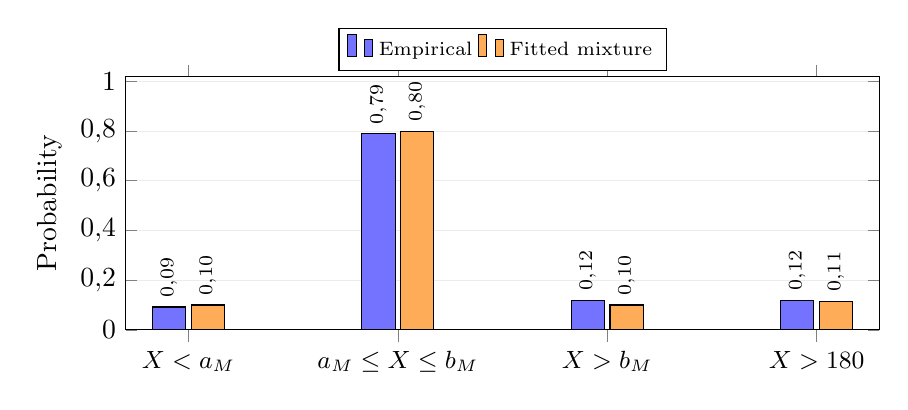
\begin{tikzpicture}
\begin{axis}[width=.92\linewidth,height=4.8cm,ybar,bar width=12pt,
ymin=0,ymax=1.02,xtick={1,2,3,4},
xticklabels={$X<a_M$,$a_M\le X\le b_M$,$X>b_M$,$X>180$},
xticklabel style={font=\small},ylabel={Probability},ytick={0,.2,.4,.6,.8,1},
legend style={at={(.5,1.02)},anchor=south,legend columns=2,font=\scriptsize},
nodes near coords,node near coords style={font=\scriptsize,rotate=90,anchor=west,
/pgf/number format/.cd,fixed,fixed zerofill,precision=2},
ymajorgrids,grid style={gray!15}]
\addplot[fill=blue!55] coordinates {(1,0.0917431192661) (2,0.788990825688) (3,0.119266055046) (4,0.119266055046)};
\addplot[fill=orange!65] coordinates {(1,0.1) (2,0.8) (3,0.1) (4,0.114420721098)};
\legend{Empirical,Fitted mixture}
\end{axis}
\end{tikzpicture}
\caption{Paired mixture probabilities at matching endpoints from
Table~\ref{tab:mixprob}; labels show two decimals, as in Figure~\ref{fig:probs}.}
\label{fig:mixprobs}
\end{figure}

\begin{figure}[htbp]
\centering
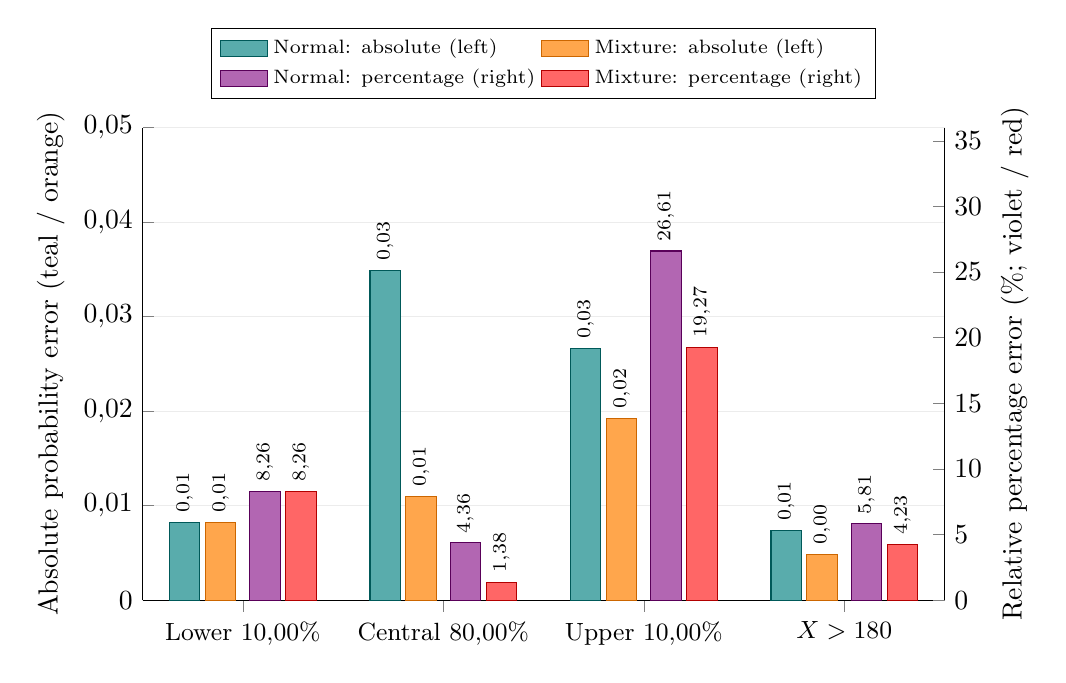
\begin{tikzpicture}
\begin{axis}[
width=.84\linewidth,height=6cm,scale only axis,
xmin=.5,xmax=4.5,ymin=0,ymax=.05,
axis y line*=left,axis x line*=bottom,
xtick={1,2,3,4},
xticklabels={Lower \displaynum{10}\%,Central \displaynum{80}\%,Upper \displaynum{10}\%,$X>180$},
xticklabel style={font=\small},
ylabel={Absolute probability error (teal / orange)},
ytick={0,.01,.02,.03,.04,.05},scaled y ticks=false,
yticklabel style={/pgf/number format/fixed},
ybar,bar width=11pt,
nodes near coords,
node near coords style={font=\scriptsize,rotate=90,anchor=west,
/pgf/number format/.cd,fixed,fixed zerofill,precision=2},
ymajorgrids,grid style={gray!15},
legend style={at={(.5,1.06)},anchor=south,legend columns=2,
font=\scriptsize,cells={anchor=west}}]
\addplot[area legend,fill=teal!65,draw=teal!70!black,bar shift=-21pt]
coordinates {(1,.008256874059)
					(2,.034862379321)
					(3,.026605504587)
					(4,.007354381954)};
\addlegendentry{Normal: absolute (left)}
\addplot[area legend,fill=orange!70,draw=orange!80!black,bar shift=-8pt]
coordinates {(1,0.0082568807339448) (2,0.011009174311939) (3,0.019266055045884) (4,0.0048453339478716)};
\addlegendentry{Mixture: absolute (left)}
\addlegendimage{area legend,fill=violet!60,draw=violet!70!black}
\addlegendentry{Normal: percentage (right)}
\addlegendimage{area legend,fill=red!60,draw=red!70!black}
\addlegendentry{Mixture: percentage (right)}
\end{axis}
\begin{axis}[
width=.84\linewidth,height=6cm,scale only axis,
xmin=.5,xmax=4.5,ymin=0,ymax=36,
axis y line*=right,axis x line=none,xtick=\empty,
ylabel={Relative percentage error (\%; violet / red)},
ytick={0,5,10,15,20,25,30,35},scaled y ticks=false,
yticklabel style={/pgf/number format/fixed},
ybar,bar width=11pt,
nodes near coords,
node near coords style={font=\scriptsize,rotate=90,anchor=west,
/pgf/number format/.cd,fixed,fixed zerofill,precision=2}]
\addplot[fill=violet!60,draw=violet!70!black,bar shift=8pt]
coordinates {(1,8.256874610091)
					(2,4.357797382454)
					(3,26.605504587156)
					(4,5.808210845243)};
\addplot[fill=red!60,draw=red!70!black,bar shift=21pt]
coordinates {(1,8.2568807339448) (2,1.3761467889923) (3,19.266055045886) (4,4.2346647542289)};
\end{axis}
\end{tikzpicture}
\caption{Errors for the normal fit (Table~\ref{tab:prob}) and the
skew-normal mixture (Table~\ref{tab:mixprob}), grouped by event.
Each four-bar group contains two close pairs: normal and mixture absolute
errors (teal and orange, left scale), then normal and mixture percentage
errors (violet and red, right scale). The normal colors match
Figure~\ref{fig:errors}. Heights across the two scales are not directly
comparable. The first three groups use each model's own quantile boundaries
($a,b$ for the normal; $a_M,b_M$ for the mixture), so they concern different
numerical events. Only $X>180$ uses the same threshold in both models.
Bar heights use unrounded errors; labels show two decimal places for both
absolute and percentage errors.}
\label{fig:mixerrors}
\end{figure}

\paragraph{Errors in model moments.}
For each moment $T$ (mean, variance or SD), use the sample statistic as the
reference and define
\[
 E_{A,T}=|T_{\mathrm{model}}-T_{\mathrm{sample}}|,\qquad
 E_{\%,T}=100\frac{E_{A,T}}{|T_{\mathrm{sample}}|}\%.
\]
These moment percentage errors use the sample reference; the probability
percentage errors above use the model probability as their reference.
Figure~\ref{fig:mixmomenterrors} compares the moments in
Table~\ref{tab:mixmoments} using full-precision values.

\begin{figure}[htbp]
\centering
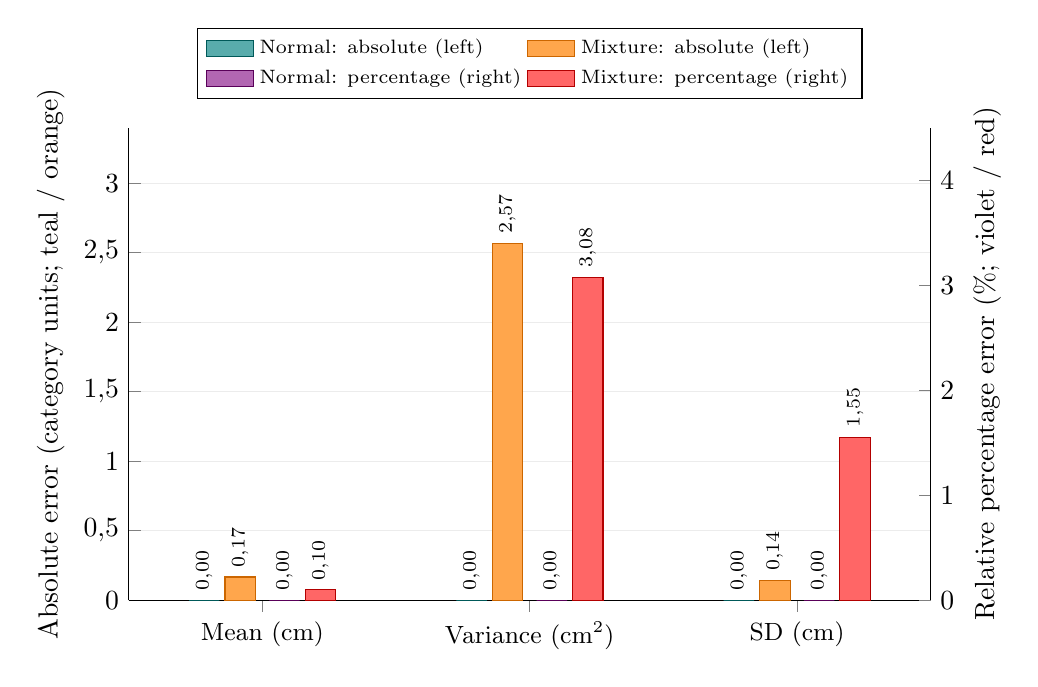
\begin{tikzpicture}
\begin{axis}[
width=.84\linewidth,height=6cm,scale only axis,
xmin=.5,xmax=3.5,ymin=0,ymax=3.4,
axis y line*=left,axis x line*=bottom,
xtick={1,2,3},
xticklabels={Mean (cm),Variance ($\mathrm{cm}^2$),SD (cm)},
xticklabel style={font=\small},
ylabel={Absolute error (category units; teal / orange)},
ytick={0,.5,1,1.5,2,2.5,3},scaled y ticks=false,
yticklabel style={/pgf/number format/fixed},
ybar,bar width=11pt,
nodes near coords,
node near coords style={font=\scriptsize,rotate=90,anchor=west,
/pgf/number format/.cd,fixed,fixed zerofill,precision=2},
ymajorgrids,grid style={gray!15},
legend style={at={(.5,1.06)},anchor=south,legend columns=2,
font=\scriptsize,cells={anchor=west}}]
\addplot[area legend,fill=teal!65,draw=teal!70!black,bar shift=-21pt]
coordinates {(1,0) (2,0) (3,0)};
\addlegendentry{Normal: absolute (left)}
\addplot[area legend,fill=orange!70,draw=orange!80!black,bar shift=-8pt]
coordinates {(1,0.16656396994952) (2,2.5671557141398) (3,0.14162451705735)};
\addlegendentry{Mixture: absolute (left)}
\addlegendimage{area legend,fill=violet!60,draw=violet!70!black}
\addlegendentry{Normal: percentage (right)}
\addlegendimage{area legend,fill=red!60,draw=red!70!black}
\addlegendentry{Mixture: percentage (right)}
\end{axis}
\begin{axis}[
width=.84\linewidth,height=6cm,scale only axis,
xmin=.5,xmax=3.5,ymin=0,ymax=4.5,
axis y line*=right,axis x line=none,xtick=\empty,
ylabel={Relative percentage error (\%; violet / red)},
ytick={0,1,2,3,4},scaled y ticks=false,
yticklabel style={/pgf/number format/fixed},
ybar,bar width=11pt,
nodes near coords,
node near coords style={font=\scriptsize,rotate=90,anchor=west,
/pgf/number format/.cd,fixed,fixed zerofill,precision=2}]
\addplot[fill=violet!60,draw=violet!70!black,bar shift=8pt]
coordinates {(1,0) (2,0) (3,0)};
\addplot[fill=red!60,draw=red!70!black,bar shift=21pt]
coordinates {(1,0.098230611251172) (2,3.0769797960448) (3,1.5505103091157)};
\end{axis}
\end{tikzpicture}
\caption{Errors in the model mean, variance and SD relative to the sample
statistics. Each group contains two close pairs: normal and mixture absolute
errors (teal and orange, left scale), then normal and mixture percentage
errors (violet and red, right scale), matching Figure~\ref{fig:mixerrors}.
The normal errors are zero by construction because its parameters use the
sample mean and SD; this is not independent evidence of fit.
Absolute errors have the units shown for each category (cm for mean and SD;
$\mathrm{cm}^2$ for variance), so their heights across categories measure
different quantities. The right scale shows percentage errors on a common
relative scale; heights across the left and right scales are not directly
comparable. Labels show two decimal places for absolute and
percentage errors.}
\label{fig:mixmomenterrors}
\end{figure}


The mixture's central-region absolute difference is 0.011009, compared
with the normal's 0.034862 at its different boundaries. This does not
compare identical events. At the shared 180 cm threshold, the mixture
gives $P_M(X>180)=0.114421$, compared with 0.126620 for
the normal and $13/109=0.119266$ empirically. Both estimates are close
to the observed proportion; the mixture has the smaller absolute difference
at this threshold.

The mixture can describe asymmetry and two peaks, but the second shape
parameter reaches the fitted bound ($\alpha_2=20$), so its sharp features
depend on a modeling constraint. Its components do not establish demographic
groups. Rounded heights, unknown sampling and measurement procedures,
and using the same data for fitting and checking limit interpretation.
In-sample agreement does not establish predictive superiority or make
the mixture the preferred model.

\end{document}
